The centers and radii of the two circles without any loss of generality are given in Table \ref{constr/55/tab:table1}
%
\begin{table}[!ht]
\begin{center}
\begin{tabular}{ | m{2cm} | m{2cm} | m{2cm} |} 
\hline
 & Circle 1 & Circle 2 \\
\hline
Centre  & $\vec{A}$=\myvec{0\\0} & $\vec{B}$=\myvec{3\\0} \\ 
\hline
Radius & $r_{1}=r_{2}=3$  \\ 
\hline
\end{tabular}
\end{center}
\caption{Input values}
\label{constr/55/tab:table1}

\end{table}

% The choice for $\vec{A}$ and $\vec{B}$ is valid as:
% \begin{align}
% \norm{\vec{B}-\vec{A}} = \norm{\vec{A}-\vec{B}}=\norm{\vec{B}}  = 3 \quad \brak{\because \vec{A}=0}
% \end{align}

Let 
\begin{align}
\vec{u}=\myvec{\cos \theta\\  \sin \theta},  \theta \in \sbrak{0,2\pi}.
\end{align}

Then on Circle 1  and Circle 2 are  given by 
\begin{align}
\vec{x}&=\vec{A}+r\vec{u}
\\
\vec{x}&=\vec{B}+r\vec{u}
\end{align}

Fig. \ref{constr/55/fig:circle} is plotted using the above equations.
%
\begin{figure}[!ht]
\centering
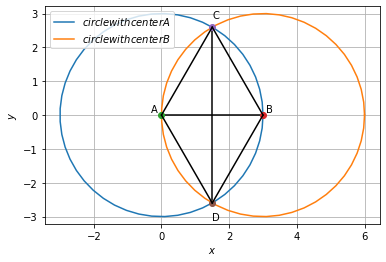
\includegraphics[width=\columnwidth]{solutions/55/Figures/figure3.png}
\caption{Circles with their points of intersection}
\label{constr/55/fig:circle}	
\end{figure}
Fig. \ref{constr/55/fig:circle} 

The general equation of Circle 1 is given by 
\begin{align}
    \norm{\vec{x}-\vec{A}}^2 &= r^2
    \\
\vec{x}^{\top}\vec{x} - 2\vec{A}^{\top}\vec{x} + \norm{\vec{A}}^2 -r_{1}^2 &= 0\label{constr/55/eq:14}
\end{align}
Similarly, for Circle 2,
\begin{align}
\vec{x}^{\top}\vec{x} - 2\vec{B}^{\top}\vec{x} + \norm{\vec{B}}^2 -r_{2}^2 = 0\label{constr/55/eq:15}
\end{align}
Subtracting \eqref{constr/55/eq:15} from \eqref{constr/55/eq:14},
\begin{align}
2\vec{B}^{\top}\vec{x}=\norm{\vec{B}}^2
\\
\myvec{1&0}\vec{x}=\frac{3}{2}
\end{align}
which can be expressed as
\begin{align}
\vec{x} &=\frac{1}{2}\myvec{3\\ 0} + \lambda \myvec{0\\1}\label{constr/55/eq:19}\\
&=\vec{q}+\lambda\vec{m} \text{ where}\label{constr/55/eq:20}\\
\vec{q}&=\myvec{1.5\\ 0},
\vec{m}=\myvec{0\\1}
\end{align}
Substituting \eqref{constr/55/eq:20} in \eqref{constr/55/eq:14}
\begin{align}
\norm{\vec{x}}^2=r^2\quad \brak{\because \vec{A}=0}
\\
\norm{\vec{q}+\lambda\vec{m}}^2=r^2\\
(\vec{q}+\lambda \vec{m})^{\top}(\vec{q}+\lambda \vec{m})=r^2\\
\implies \vec{q}^{\top}(\vec{q}+\lambda \vec{m})+\lambda \vec{m}^{\top}(\vec{q}+\lambda \vec{m})=r^2
\\
\implies \norm{\vec{q}}^2+\lambda\vec{q}^{\top}\vec{m}+\lambda\vec{m}^{\top}\vec{q}+\lambda^2\norm{\vec{m}}^2=r^2
\\
\implies \norm{\vec{q}}^2+2\lambda\vec{q}^{\top}\vec{m}+\lambda^2\norm{\vec{m}}^2=r^2 
% \\
% \implies \lambda(\lambda\norm{\vec{m}}^2+2\vec{q}^{\top}\vec{m})=r^2-\norm{\vec{q}}^2\\
% \implies\lambda^2\norm{\vec{m}}^2=9-\norm{\vec{q}}^2
\\
\implies \lambda=\pm \sqrt{\frac{9-\norm{\vec{q}}^2}{\norm{\vec{m}}^2}} \quad \because \vec{q}^{\top}\vec{m} = 0
% \lambda^2=6.75\\
% \lambda=+\sqrt{6.75},-\sqrt{6.75}
\end{align}
Substituting the value of $\lambda$ in \eqref{constr/55/eq:20},
\begin{align}
%\vec{x}=\vec{q}+\lambda\vec{m}\\
\vec{C}&=\vec{q}+\lambda\vec{m}\\
\vec{D}&=\vec{q}-\lambda\vec{m} \\
\implies (\vec{A}-\vec{B})^{\top}(\vec{C}-\vec{D})
&=2\myvec{-3&0}\myvec{0\\\sqrt{6.75}}
\\
&=0
\\
\implies AB\perp CD
\end{align}


% We have $\vec{C}$ and $\vec{D}$ as points of intersection and $r_{1}=r_{2}$.So,
% \begin{align}
% \norm{\vec{C}-\vec{A}}^2 = \norm{\vec{C}-\vec{B}}^2
% \end{align}
% \begin{align}
% \implies(\vec{C}-\vec{A})^{\top}(\vec{C}-\vec{A})=(\vec{C}-\vec{B})^{\top}(\vec{C}-\vec{B})
% \\
% \implies \vec{A}^{\top}\vec{C}-\vec{B}^{\top}\vec{C}=\vec{C}^{\top}\vec{B}-\vec{C}^{\top}\vec{A}+\norm{\vec{A}}^2-\norm{\vec{B}}^2 
% \end{align}
% \begin{align}
% \implies2\times \vec{A}^{\top}\vec{C}-2\times\vec{B}^{\top}\vec{C}=\norm{\vec{A}}^2-\norm{\vec{B}}^2 \label{constr/55/eq:1}
% \end{align}
% Similarly,using:
% \begin{align}
% \norm{\vec{D}-\vec{A}}^2 = \norm{\vec{D}-\vec{B}}^2
% \end{align}
% We get:
% \begin{align}
% 2\times \vec{A}^{\top}\vec{D}-2\times\vec{B}^{\top}\vec{D}=\norm{\vec{A}}^2-\norm{\vec{B}}^2 \label{constr/55/eq:2}
% \end{align}

% Subtracting equation \ref{constr/55/eq:2} from equation \ref{constr/55/eq:1}:
% \begin{align}
% 2\times(\vec{A}^{\top}-\vec{B}^{\top})(\vec{C}-\vec{D})=0
% \\
% \implies (\vec{A}-\vec{B})^{\top}(\vec{C}-\vec{D})=0
% \\
% \implies AB\perp CD
% \end{align}
